% ============================================================
%  ML IoT Lab – Presentation Template
%  HCMUT EE Machine Learning & IoT Lab
%  Faculty of Electrical & Electronics Engineering, HCMUT
%
%  Usage: compile with pdflatex (twice) or xelatex
% ============================================================

\documentclass[aspectratio=169, 10pt]{beamer}
\usepackage{newtxtext}
\usepackage{newtxmath}
\usepackage{beamerthemeMLIOT}   % custom theme (in same folder)




% ---- Additional packages ----
\usepackage{amsmath, amssymb}
\usepackage{booktabs}
\usepackage{multicol}
\usepackage{caption}
\usepackage{hyperref}
\usepackage[loadonly]{enumitem}
\usepackage{array}
\usepackage{pifont}
\usepackage{ragged2e}
\usepackage{graphicx}

% ---- Hyperlink colours ----
\hypersetup{
  colorlinks = true,
  urlcolor   = MLIOTaccent,
  linkcolor  = MLIOTblue,
  citecolor  = MLIOTblue
}

% ============================================================
%  PAPER METADATA – fill these in
% ============================================================
\title{Multi-Sensor Smart Irrigation System.}

\author{%
  \textbf{\textcolor{MLIOTaccent}{Author 1}}%
  \texorpdfstring{\textcolor{MLIOTgold}{\textsuperscript{*a}}}{*a}\textcolor{MLIOTnavy}{,~}%
  \textbf{\textcolor{MLIOTnavy}{Author 2}}%
  \texorpdfstring{\textcolor{MLIOTgold}{\textsuperscript{a}}}{a}\textcolor{MLIOTnavy}{,~}%
  \textbf{\textcolor{MLIOTnavy}{Author 3}}%
  \texorpdfstring{\textcolor{MLIOTgold}{\textsuperscript{b}}}{b}%
}


\setAffiliations{%
  \textsuperscript{a}Author Affiliation \\
  \textsuperscript{b}Co-author Affiliation%
}

\setCorrespondingAuthor{%
  *Corresponding/Presenting Author Email: \href{mailto:author@mail.com}{author@mail.com}%
}

\setPaperID{MLIOT-2026-XXX}

\institute{%
  Machine Learning \& IoT Lab,
  Ho Chi Minh City University of Technology (HCMUT)%
}

\date{June 2026}



% ============================================================
\begin{document}
% ============================================================

% ------------------------------------------------------------
%  SLIDE 1 – Title Slide
% ------------------------------------------------------------
\begin{frame}[plain]
  \titlepage
\end{frame}

% ------------------------------------------------------------
%  SLIDE 2 – Outline
% ------------------------------------------------------------
\begin{frame}{Outline}
	\begin{columns}[T]
		\begin{column}{0.55\textwidth}
			% This temporary font assignment scales the numbers perfectly
			\setbeamerfont{enumerate item}{size=\large}
			
			\begin{enumerate}
				\setlength{\itemsep}{0.8em} % Keeps a comfortable gap between items
				\item {\large Introduction} 
				\item {\large Objectives} 
				\item {\large Methodology} 
				\item {\large Results and Discussion} 
				\item {\large Conclusions} 
				\item {\large References} 
			\end{enumerate}
		\end{column}
		\begin{column}{0.42\textwidth}
			\begin{block}{Contact Information}
				\footnotesize
				\textbf{\textcolor{MLIOTnavy}{Address:}}~403.1 BK.B6, HCMUT Campus 2\\[0.35em]
				\textbf{\textcolor{MLIOTnavy}{Email:}}\\
				nkloi@hcmut.edu.vn\\
				mlandiotlab@gmail.com\\[0.35em]
				\textbf{\textcolor{MLIOTnavy}{Website:}}~mliotlab.com\\[0.35em]
				\textbf{\textcolor{MLIOTnavy}{Facebook:}}~facebook.com/hcmut.ml.iot.lab\\[0.35em]
				\textbf{\textcolor{MLIOTnavy}{YouTube:}}~youtube.com/@mliotlab
			\end{block}
		\end{column}
	\end{columns}
\end{frame}

% ------------------------------------------------------------
%  SLIDE 3 – Introduction
% ------------------------------------------------------------
\begin{frame}{Introduction}
  \begin{columns}[T]
    % Left column – Background / Motivation
    \begin{column}{0.52\textwidth}
      \begin{block}{Problem Statement}
        \begin{itemize}
          \item wasting water.
          \item Dependent on human presence.
          \item Insufficient data for decision - making.
          \item Water stress due to insufficient or exessive watering
        \end{itemize}
      \end{block}
    \end{column}
    % Right column – Literature Review Highlights
     \begin{column}{0.45\textwidth}
      \begin{block}{Literature Review Highlights}
        \begin{itemize}
          \item Author et al.\ (Year): Key finding 1.\cite{ref1}
          \item Author et al.\ (Year): Key finding 2.\cite{ref2}
        \end{itemize}
        \vspace{0.5em}
        \textbf{\textcolor{MLIOTcoral}{Research Gap:}}
        \textit{Describe gap identified.}
      \end{block}
    \end{column}
  \end{columns}
\end{frame}

% ------------------------------------------------------------
%  SLIDE 4 – Additional Content Slide
%  (Blank content slide — customise as needed)
% ------------------------------------------------------------
\begin{frame}{Content Slide}
  \begin{itemize}
      \item Total presentation time: \textbf{10 minutes} (strictly enforced)
      \item Questions \& Answers: 2 minutes
      \item Please adhere strictly to the allotted time.
      \item Keep slides clear, concise, and visually clean.
      \item Use readable font sizes.
      \item Maintain consistent formatting throughout the presentation.
      \item Use high-quality figures, graphs, and images.
      \item Ensure all plots/figures have proper labels and units.
      \item Avoid overcrowding slides.
      \item Videos/animations should be brief and relevant.
      \item Cite references wherever.
  \end{itemize}
\end{frame}

% ------------------------------------------------------------
%  SLIDE 5 – DHT11
% ------------------------------------------------------------
\begin{frame}{DHT11 sensor}
  \begin{columns}[c] % [c] để căn giữa nội dung 2 cột theo chiều dọc

    % Cột bên trái: Dùng cho Hình ảnh (chiếm 45% chiều rộng slide)
    \begin{column}{0.45\textwidth}
      \centering
      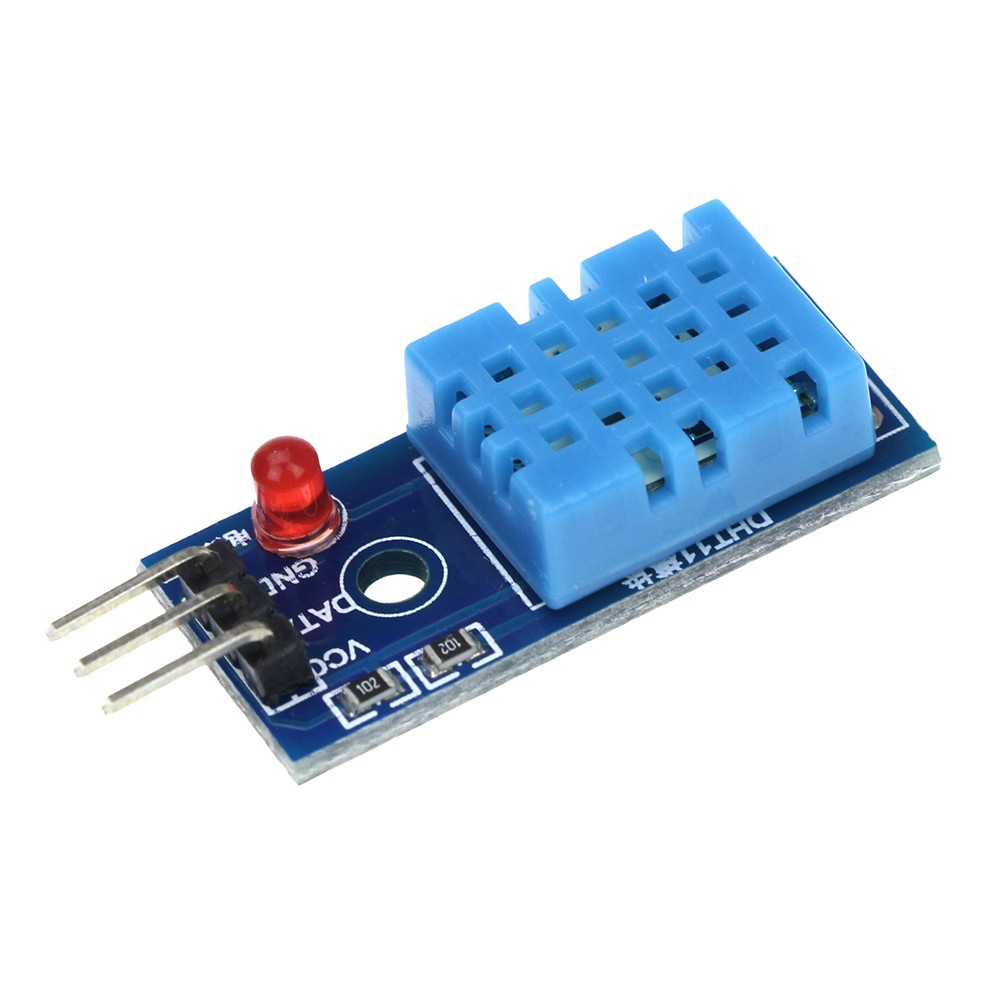
\includegraphics[width=\textwidth]{image/dht11.jpg}
      \vspace{0.3em}
      {\footnotesize\textit{Fig 1: DHT11 sensor}}
    \end{column}

    % Cột bên phải: Dùng cho Văn bản / Đặc tính (chiếm 50% chiều rộng slide)
    \begin{column}{0.50\textwidth}
      \begin{block}{Technical specifications}
        \begin{itemize}
          \item \textbf{Measurement range:} 20 -- 90\%RH, 0 -- 50$^\circ$C
          \item \textbf{Humidity Accuracy:} $\pm$ 5\%
          \item \textbf{Temperature Accuracy:} $\pm$ 2\%
          \item \textbf{Communication Standard:} 1-Wire (Single Bus)
        \end{itemize}
      \end{block}
    \end{column}

  \end{columns}
\end{frame}

% ------------------------------------------------------------
%  SLIDE 6 – Communication Process of the DHT11
% ------------------------------------------------------------

\begin{frame}{Communication Process of the DHT11}
  \begin{columns}[c]
    
    % --- CỘT BÊN TRÁI (Chứa Hình Trên-Trái và Hình Dưới-Trái) ---
    \begin{column}{0.48\textwidth}
      \centering
      % Hình 1: Trên - Trái
      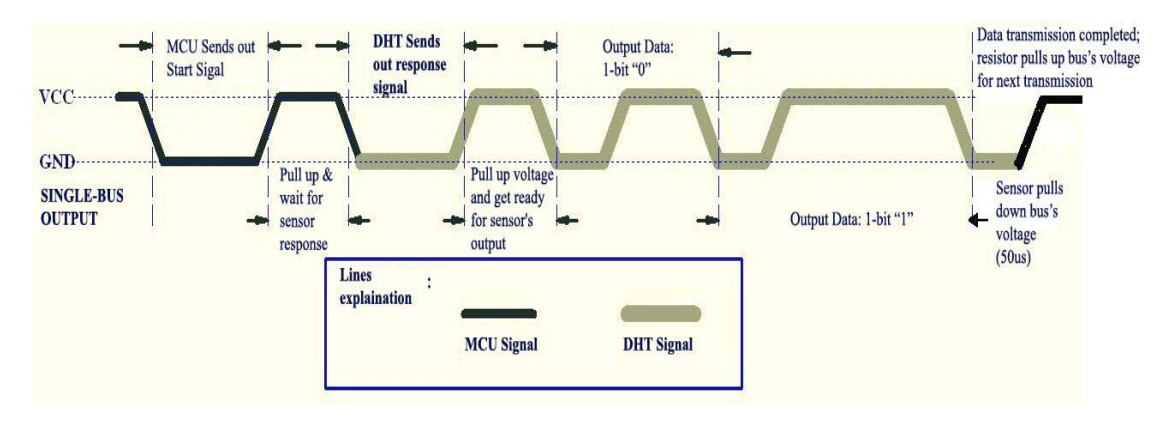
\includegraphics[height=0.35\textheight]{image/OverallCommunicationProcess.png}\\
      {\tiny\textit{Fig 1: Overall Communication Process}}\\[0.6em]

      % Hình 2: Dưới - Trái
    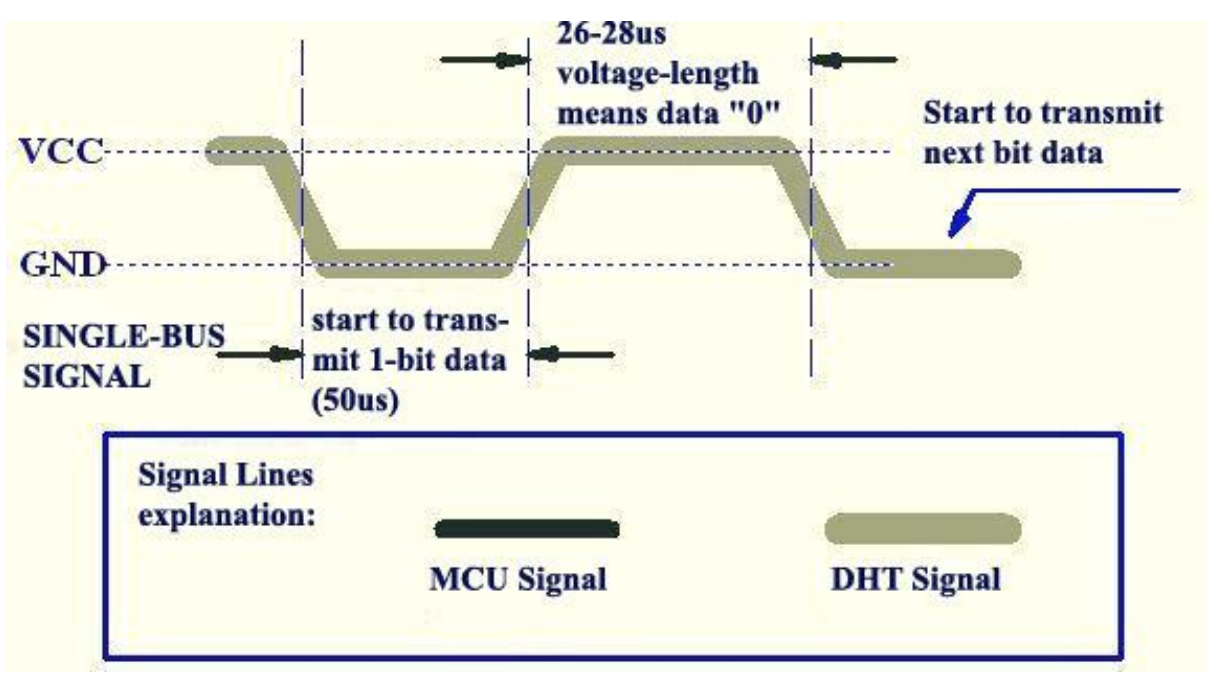
\includegraphics[height=0.35\textheight]{image/DHT11_Data0.png}\\
      {\tiny\textit{Fig 3:  Data "0" Indication}}\\
      
    \end{column}

    % --- CỘT BÊN PHẢI (Chứa Hình Trên-Phải và Hình Dưới-Phải) ---
    \begin{column}{0.48\textwidth}
      \centering
      % Hình 3: Trên - Phải
      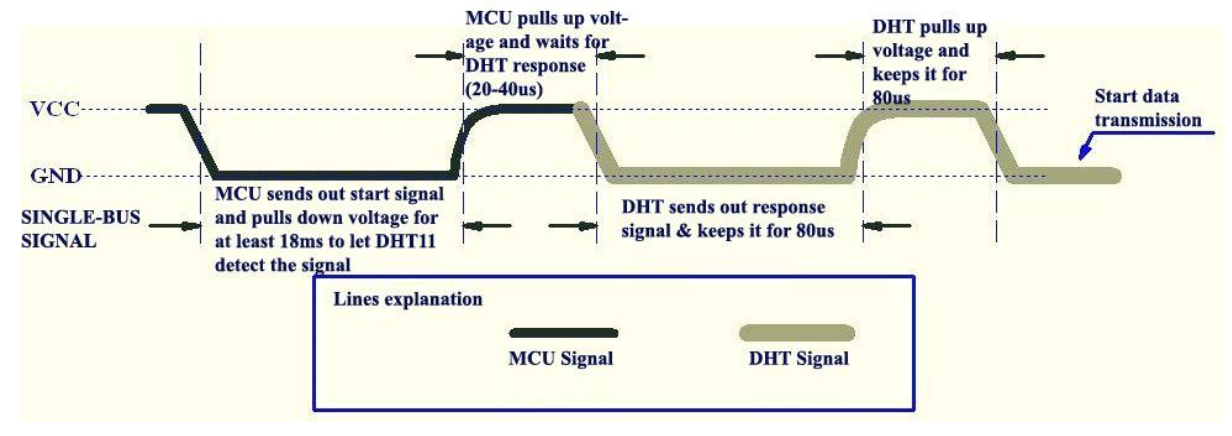
\includegraphics[height=0.35\textheight]{image/MCUSendsout StartSignal&DHTResponses.png}\\
      {\tiny\textit{Fig 2:  MCU Sends out Start Signal and DHT Responses}}\\[0.6em]

      % Hình 4: Dưới - Phải
      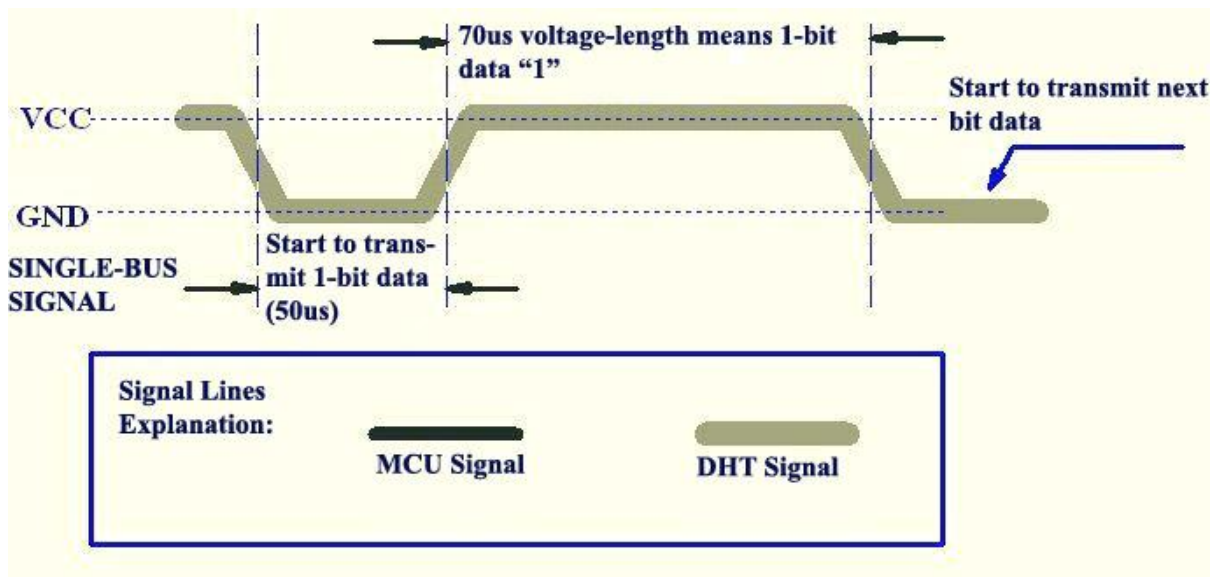
\includegraphics[height=0.35\textheight]{image/DHT11_Data1.png}\\
      {\tiny\textit{Fig 4:  Data "1" Indication}}
    \end{column}

  \end{columns}
\end{frame}

% ------------------------------------------------------------
%  SLIDE 7 – BH1750
% ------------------------------------------------------------
\begin{frame}{Light sensor BH1750}
  \begin{columns}[c]
        \begin{column}{0.45\textwidth}
      \centering
      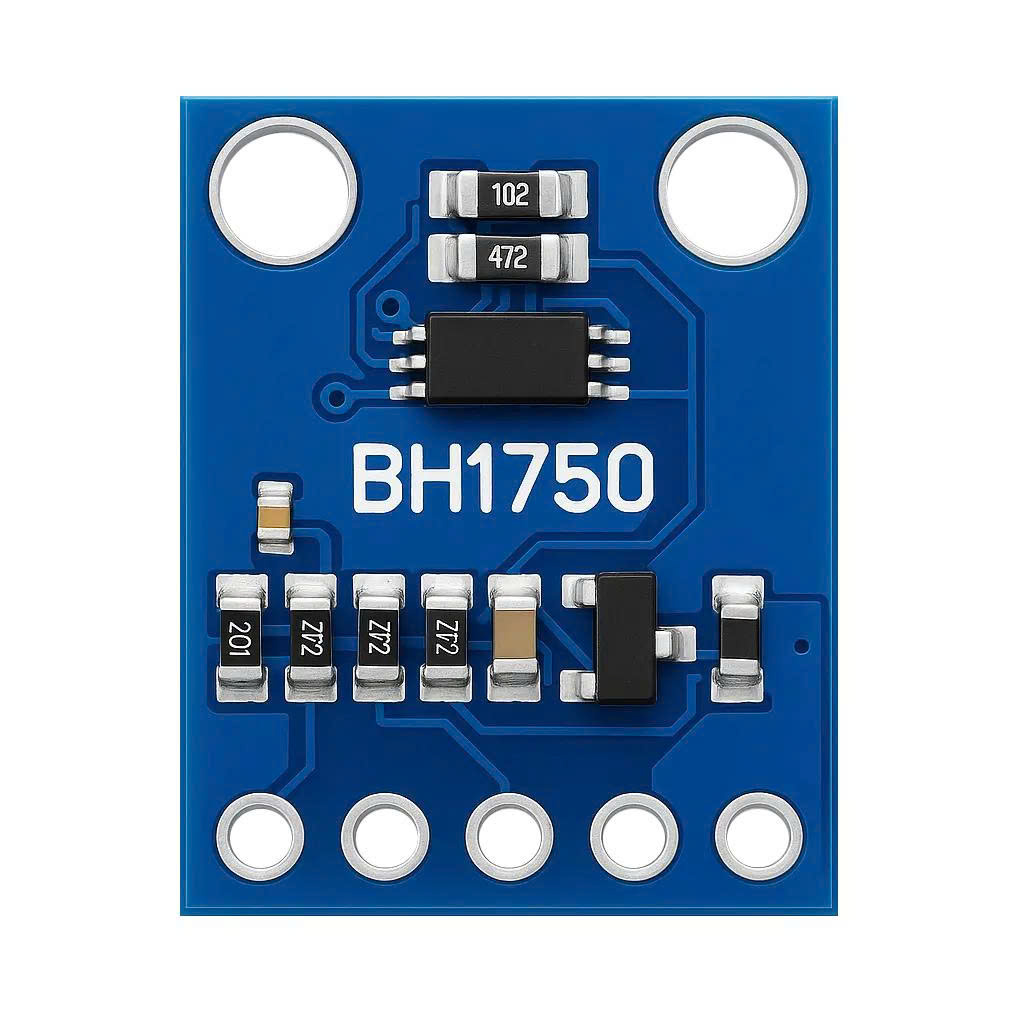
\includegraphics[width=\textwidth]{image/bh1750.jpg}
      \vspace{0.3em}
      {\footnotesize\textit{Fig 1: BH2750}}
    \end{column}

    \begin{column}{0.50\textwidth}
      \begin{block}{Features}
        \begin{itemize} 
          \item \textbf{I2C bus interface}
          \item \textbf{Illuminance to Digital Converter}
          \item \textbf{Wide range and High resolution: }1 -- 65535 lx
          \item \textbf{Small measurement variation: }$\pm$20\%
          \item \textbf{ 2 type of I2C slave-address: }H -- 0x5C, L -- 0x23
          \item \textbf{...}
        \end{itemize}
      \end{block}
    \end{column}
  \end{columns}
\end{frame}

% ------------------------------------------------------------
%  SLIDE 8 – How to program the BH1750 sensor
% ------------------------------------------------------------

\begin{frame}{How to program the BH1750 sensor}
  \begin{columns}[c]
    \begin{column}{0.45\textwidth}
      \begin{block}{Programing BH1750 sensor}
        \begin{enumerate}
            \item \textbf{Configure RCC: }GPIO, I2C
            \item \textbf{Send command: }Send slave address, Opcode
            \item \textbf{Read data: }Combine those two bytes and divide by the factor 1.2.
        \end{enumerate}
      \end{block}
    \end{column}
    \begin{column}{0.5\textwidth}
      \centering
      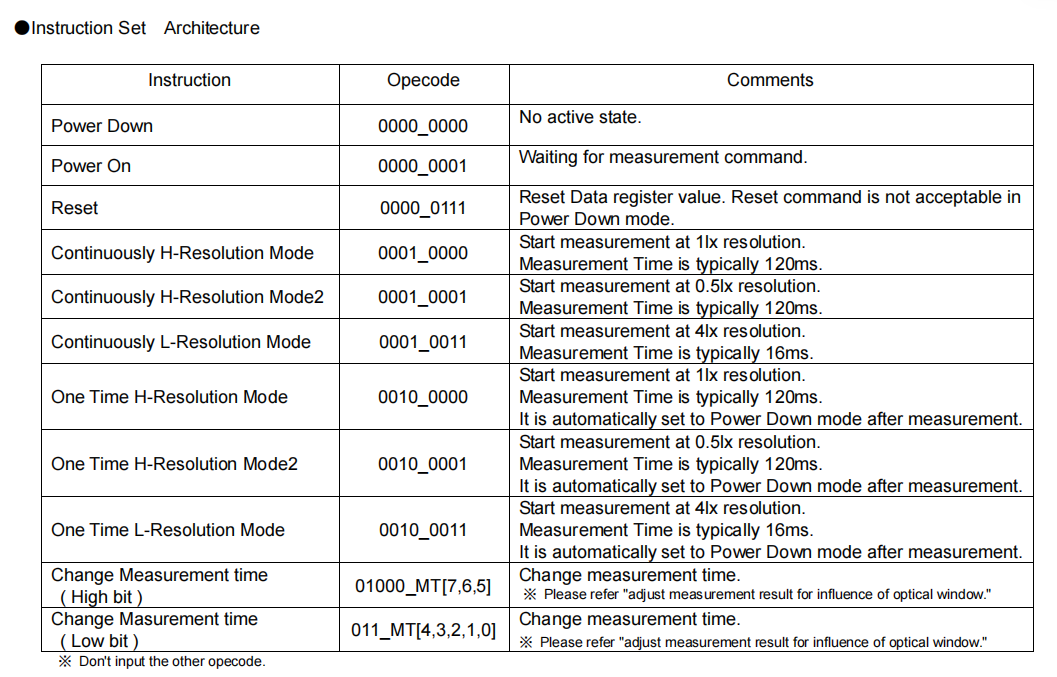
\includegraphics[width=\textwidth]{image/opcode_bh1750.png}
      \vspace{0.3em}
      {\footnotesize\textit{Fig 1: Instruction Set Architecture}}
    \end{column}
  \end{columns}
\end{frame}

% ------------------------------------------------------------
%  SLIDE 9-Aim and Objectives
% ------------------------------------------------------------
\begin{frame}{Objectives}
\begin{itemize}
    \item Data acquisition and processing.
    \item Automatic control.
    \item User interface and monitoring.
    \item Reliability and safety.
    \item Project deliverables he Study.
\end{itemize}
\end{frame}

% ------------------------------------------------------------
%  SLIDE 10 Methodology
% ------------------------------------------------------------
\begin{frame}{Methodology}
  \begin{methodcols}
    \methodcol{\ding{202}~Problem Setup}{%
      \begin{itemize}
        \item Indentify the problem of inefficient irrigation.
        \item Monitor soil and environmental conditions using multiple sensor.
        \item Define system inputs, outputs and operating conditions.
      \end{itemize}%
    }
    \methodcol{\ding{203}~Governing Equations}{%
      \begin{itemize}
        \item Define sensor thresholds for irrigation decisions.
        \item Establish the control logic for automatic irrigation.
        \item Set conditions for turning the water pump ON/OFF.
      \end{itemize}%
    }
    \methodcol{\ding{204}~Numerical / Experimental Method}{%
      \begin{itemize}
        \item Cellect and process data from multiple sensor.
        \item Implement automatic irrigation using STM32 and relay control.
        \item Test and validate the system under different soil moisture conditions.
      \end{itemize}%
    }
  \end{methodcols}

  \vspace{0.4em}
  \begin{center}
    \begin{beamercolorbox}[wd=0.65\textwidth, rounded=true, sep=5pt,
          center]{block body}
      \textit{\small Multi-Sensor Data --> Data processing --> Decision making --> Relay control --> Water pump --> Monitoring}
    \end{beamercolorbox}
  \end{center}
\end{frame}

% ------------------------------------------------------------
%  SLIDE 11 Results and Discussion
% ------------------------------------------------------------
\begin{frame}{Results and Discussion}
  \begin{columns}[T]
    \begin{column}{0.48\textwidth}
      \begin{beamercolorbox}[wd=\textwidth, rounded=true, sep=5pt,
            center]{block body}
        \vspace{1.8cm}
        \textit{\small Insert Figure / Contour Plot / Chart Here}
        \vspace{1.8cm}
      \end{beamercolorbox}
      \vspace{0.3em}
      {\footnotesize\textit{Fig.~1: Caption describing the figure in detail.}}
    \end{column}
    \begin{column}{0.48\textwidth}
      \begin{block}{\textcolor{MLIOTwhite}{Key Observations}}
        \begin{itemize}
          \item Finding / observation 1 from the results.
          \item Finding / observation 2 with quantitative value.
          \item Comparison with literature / benchmark values.
          \item Physical interpretation of observed trends.
        \end{itemize}
      \end{block}
    \end{column}
  \end{columns}
\end{frame}


\begin{frame}{Results and Discussion}
  \begin{columns}[T]
    \begin{column}{0.48\textwidth}
      \begin{beamercolorbox}[wd=\textwidth, rounded=true, sep=5pt,
            center]{block body}
        \vspace{1.8cm}
        \textit{\small Insert Figure / Contour Plot / Chart Here}
        \vspace{1.8cm}
      \end{beamercolorbox}
      \vspace{0.3em}
      {\footnotesize\textit{Fig.~1: Caption describing the figure in detail.}}
    \end{column}
    \begin{column}{0.48\textwidth}
      \begin{block}{\textcolor{MLIOTwhite}{Key Observations}}
        \begin{itemize}
          \item Finding / observation 1 from the results.
          \item Finding / observation 2 with quantitative value.
          \item Comparison with literature / benchmark values.
          \item Physical interpretation of observed trends.
        \end{itemize}
      \end{block}
    \end{column}
  \end{columns}
\end{frame}


\begin{frame}{Results and Discussion}
  \begin{columns}[T]
    \begin{column}{0.48\textwidth}
      \begin{beamercolorbox}[wd=\textwidth, rounded=true, sep=5pt,
            center]{block body}
        \vspace{1.8cm}
        \textit{\small Insert Figure / Contour Plot / Chart Here}
        \vspace{1.8cm}
      \end{beamercolorbox}
      \vspace{0.3em}
      {\footnotesize\textit{Fig.~1: Caption describing the figure in detail.}}
    \end{column}
    \begin{column}{0.48\textwidth}
      \begin{block}{\textcolor{MLIOTwhite}{Key Observations}}
        \begin{itemize}
          \item Finding / observation 1 from the results.
          \item Finding / observation 2 with quantitative value.
          \item Comparison with literature / benchmark values.
          \item Physical interpretation of observed trends.
        \end{itemize}
      \end{block}
    \end{column}
  \end{columns}
\end{frame}

% ------------------------------------------------------------
%  SLIDE 14-Conclusions
% ------------------------------------------------------------
\begin{frame}{Conclusions}
  \footnotesize % <--- Add this command right before the itemize block!
  \begin{itemize}
    \setlength{\itemsep}{0.5em}
    \item \textbf{Conclusion 1:} The system successfully monitors soil and environmetal conditions using
          multiple sensor.
    \item \textbf{Conclusion 2:} The system automatically controls irrigation based
          on sensor data and predefined thresholds.
    \item \textbf{Conclusion 3:} Experimental results demonstrate the feasibility
          of the proposed system.
    % Add more conclusions as needed:
    % \item \textbf{Conclusion 2:} ...
  \end{itemize}

  \vspace{1em}
  \begin{beamercolorbox}[wd=\textwidth, rounded=true, sep=7pt]{block body alerted}
    \textbf{\textcolor{MLIOTblue}{Future Work:}}
    \textcolor{MLIOTink}{\footnotesize Integrate Wi-Fi connectivity and cloud services, develop
    a real-time monitoring dashboard, and incorporate AI for intelligent decision-making.}
  \end{beamercolorbox}
\end{frame}

% ------------------------------------------------------------
%  SLIDE 9 – References
% ------------------------------------------------------------
\begin{frame}{References}
  \begin{thebibliography}{9}
    \setbeamertemplate{bibliography item}[text]

    \bibitem{ref1}
    Author, A.\,B., Author, C.\,D.\ (Year).
    \textit{Title of the paper.}
    \textit{Journal Name}, Vol(Issue), pp.\,xxx--xxx.
    DOI: \href{https://doi.org/10.xxxx/xxxxx}{10.xxxx/xxxxx}

  \bibitem{ref2}
    Author, A.\,B., Author, C.\,D.\ (Year).
    \textit{Title of the paper.}
    \textit{Journal Name}, Vol(Issue), pp.\,xxx--xxx.
    DOI: \href{https://doi.org/10.xxxx/xxxxx}{10.xxxx/xxxxx}

    \bibitem{BH175_Datasheet}
    ROHM Semiconductor.\ (2009).
    \textit{Digital 16bit Serial Output Type 
Ambient Light Sensor IC}
    \textit{Datasheet Rev.\ D}, pp.\,1--18.
    DOI: \href{https://www.alldatasheet.vn/datasheet-pdf/pdf/338083/ROHM/BH1750FVI.html}{ROHM-BH1750FVI}

    \bibitem{DHT11_Datasheet}
    OSEPP Electronics.\ (2010).
    \textit{DHT11 Digital Humidity and Temperature Sensor.}
    \textit{Datasheet Rev.\ 1.0}, pp.\,1--9.
    DOI: \href{https://www.alldatasheet.com/datasheet-pdf/pdf/2193416/OSEPP/DHT11.html}{OSEPP-DHT11}
    % Add more references below as needed:
    % \bibitem{ref3} ...

  \end{thebibliography}
\end{frame}

% ------------------------------------------------------------
%  SLIDE 10 – Thank You / Acknowledgements
% ------------------------------------------------------------
\thankyouslide{%
  \textit{The authors gratefully acknowledge [Funding agency / Collaborators /
  Lab / Advisor names] for their support and guidance.}
}

% ============================================================
\end{document}
% ============================================================